\documentclass[aspectratio=169, table]{beamer}

\graphicspath{{../../images/}}
%\usepackage[beamertheme=./praditatheme]{Pradita}

\usetheme{Pradita}
\title{\huge Chapter-13:\\Container\vspace{10pt}}
\subtitle{IF231303-Software Architecture}
\author{Richwen Canady, Desfantio Wuidjaja, Vincenzo Matalino\\Alfa yohannis}
\begin{document}

    \begin{frame}[plain]
        \maketitle
    \end{frame}

    \begin{frame}
        \frametitle{What are Containers?}
        \begin{itemize}
            \item Containers are lightweight, stand-alone, executable packages that include everything needed to run a piece of software: code, runtime, system tools, libraries, and settings.
            \item They share the operating system kernel and isolate application processes from the host system and each other.
        \end{itemize}
    \end{frame}

    \begin{frame}
        \frametitle{Understanding Docker}
        \begin{itemize}
            \item Docker is a popular platform for developing, shipping, and running applications using containerization.
            \item It enables you to separate your applications from your infrastructure to deliver software quickly and reliably.
            \item Docker provides the ability to package and run an application in a loosely isolated environment called a container.
        \end{itemize}
    \end{frame}


    \begin{frame}
        \frametitle{Background and Motivation}
        \begin{itemize}
            \item \textbf{Traditional Virtualization:} Heavyweight, slower, and more resource-intensive.
            \item \textbf{Containers:} Lightweight, fast, share the host OS kernel, and require fewer resources.
            \item Need for a consistent development environment to avoid "works on my machine" issues.
            \item Facilitates microservices architecture, allowing easy deployment and scaling of applications.
        \end{itemize}
    \end{frame}


    \begin{frame}{Container vs Virtual Machine}
        \vspace{30pt}
        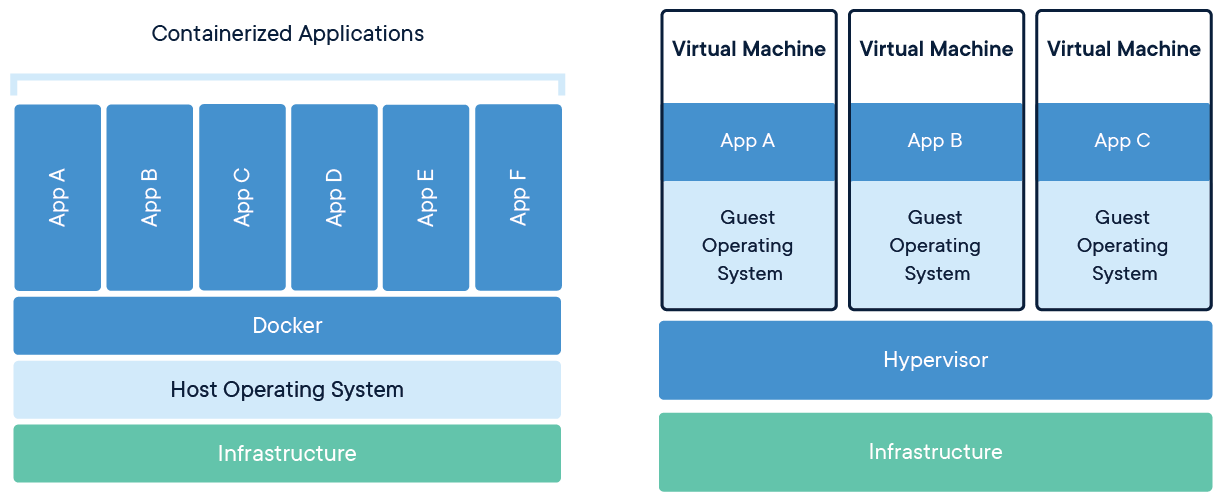
\includegraphics[width=\textwidth]{../../images/container-vm.png}
    \end{frame}


    \begin{frame}
        \frametitle{Container vs Virtual Machine}
        \vspace{25pt}
        \begin{itemize}
            \item \textbf{Virtual Machines:}
            \begin{itemize}
                \item Include the entire OS.
                \item Heavyweight and require more resources.
                \item Slower to start up.
                \item \textbf{Hypervisor:} Manages virtual machines, allowing multiple VMs to run on a single physical machine by abstracting hardware resources.
            \end{itemize}
            \item \textbf{Containers:}
            \begin{itemize}
                \item Share the host OS kernel.
                \item Lightweight and require fewer resources.
                \item Faster to start up.
            \end{itemize}
            \item Containers are ideal for microservices and DevOps practices due to their efficiency and scalability.
        \end{itemize}
    \end{frame}

     %        \framesubtitle{}
    \begin{frame}{Docker}
        \vspace{30pt}
        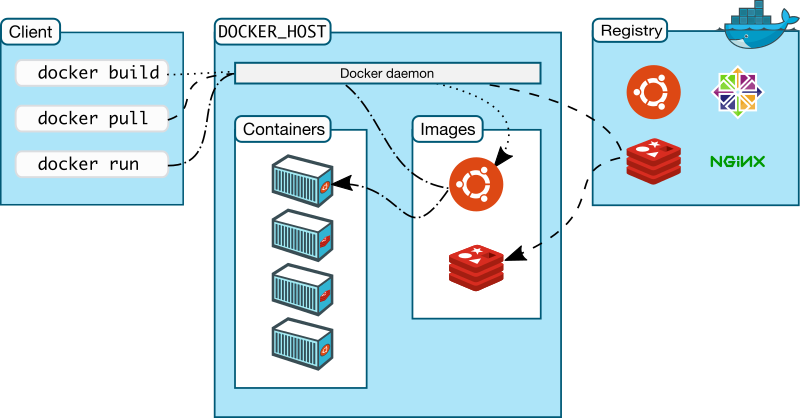
\includegraphics[width=\textwidth]{../../images/docker.png}
    \end{frame}

    \begin{frame}
        \frametitle{Components}
        \begin{itemize}
            \item \textbf{Docker Engine:} The core part of Docker, consisting of:
            \begin{itemize}
                \item \textbf{Docker Daemon:} Runs on the host machine and manages Docker containers, images, networks, and storage volumes.
                \item \textbf{Docker Client:} The command-line interface that users interact with.
            \end{itemize}
            \item \textbf{Images:} Read-only templates used to create containers.
            \item \textbf{Containers:} Runnable instances of Docker images.
            \item \textbf{Docker Registry:} Stores Docker images (e.g., Docker Hub).
        \end{itemize}
    \end{frame}

    \begin{frame}
        \frametitle{Advantages of Using Containers}
        \begin{itemize}
            \item \textbf{Portability:} Consistent environments across different platforms.
            \item \textbf{Efficiency:} Reduced overhead compared to virtual machines.
            \item \textbf{Scalability:} Easily scale up or down based on demand.
            \item \textbf{Isolation:} Applications run in isolated environments, preventing conflicts.
            \item \textbf{CI/CD:} Streamlines the process of development, testing, and deployment.
        \end{itemize}
    \end{frame}


    \begin{frame}
        \frametitle{Drawbacks of Containers}
        \begin{itemize}
            \item \textbf{Security:} Shared kernel can pose a security risk.
            \item \textbf{Persistence:} Managing stateful applications can be challenging.
            \item \textbf{Networking:} Complex networking setups can be difficult to manage.
            \item \textbf{Compatibility:} Not all applications are suited for containerization.
        \end{itemize}
    \end{frame}


    \begin{frame}
        \frametitle{Examples of Applications}
        \begin{itemize}
            \item \textbf{Web Applications:} Deploy web services with consistent environments.
            \item \textbf{Microservices:} Implement microservices architecture with isolated services.
            \item \textbf{Development Environments:} Create consistent development and testing environments.
            \item \textbf{Data Processing:} Run data processing tasks in isolated containers.
            \item \textbf{CI/CD Pipelines:} Automate the build, test, and deployment processes.
        \end{itemize}
    \end{frame}


    \begin{frame}
        \frametitle{Conclusions}
        \begin{itemize}
            \item Containers, especially with Docker, revolutionize software development and deployment.
            \item They provide lightweight, consistent, and isolated environments.
            \item While there are challenges, the benefits often outweigh the drawbacks, particularly in scalable and microservice-based architectures.
        \end{itemize}
    \end{frame}


\end{document}
